\documentclass[xcolor=table]{beamer}

\usepackage{lscape, amsmath, amsfonts, amssymb, setspace, theorem, wrapfig, graphicx, float, multirow, subfig, color, rotating, multicol, datetime, natbib, venndiagram, pstricks, xkeyval, tikz, etoolbox, verbatim, subfig}

\usepackage{listings}
\usepackage{xcolor}
\usepackage{natbib}

\definecolor{codegreen}{rgb}{0,0.6,0}
\definecolor{codegreengray}{rgb}{0,0.4,0}
\definecolor{codegray}{rgb}{0.5,0.5,0.5}
\definecolor{codeblue}{rgb}{0.00,0,0.82}
\definecolor{backcolour}{rgb}{0.95,0.95,0.92}
 
\lstdefinestyle{mystyle}{
    backgroundcolor=\color{backcolour},   
    commentstyle=\color{codegreengray},
    numberstyle=\tiny\color{codegray},
    stringstyle=\color{codegreen},    basicstyle=\ttfamily\footnotesize,
    breakatwhitespace=false,         
    breaklines=true,                 
    captionpos=b,                    
    keepspaces=true,                 
    numbers=left,                    
    numbersep=5pt,                  
    showspaces=false,                
    showstringspaces=false,
    showtabs=false,                  
    tabsize=2
}
 
\lstset{style=mystyle}

\title{GV300 - Quantitative Political Analysis}
\subtitle{University of Essex - Department of Government}
\date{Week 10 -- 2 December, 2019}				% or you can specify a date, just write it down instead of "\today"
\author{Lorenzo Crippa} 

\usetheme[progressbar=frametitle]{metropolis}
\usecolortheme{seahorse}						% try others: wolverine; crane...


\begin{document}

\frame{
\titlepage
}

\frame{
\frametitle{Regression Analysis}
\begin{center}
Today we'll work on regression analysis and apply what you have learnt in class.
We'll use the dataset on sales of Monet paintings that we have started to explore in week 8.
\end{center}
}

\frame{
\frametitle{Explaining prices of paintings -- Part 1}
Load your data of Monet paintings and perform the following steps:
\begin{enumerate}
\item Explore how variables relate to each other (bivariate \emph{descriptive} analysis)
	\begin{itemize}
	\item Use appropriate statistics to talk about these relations
	\item Use appropriate plots to show the relations
	\end{itemize}
\item Propose a theory about what explains the price of a painting
	\begin{itemize}
	\item What is your theory?
	\item What is the underlining population of your theory?
	\item What is the sample you are using?
	\end{itemize}
\item Build an appropriate linear model to test your theory
	\begin{itemize}
	\item What variables do you include?
	\item Think and justify whether you meet Gauss-Markov assumptions
	\item What could violate them?
	\item What could improve your model?
	\end{itemize}
\end{enumerate}
}

\frame{
\frametitle{Explaining prices of paintings -- Part 2}
\begin{enumerate}
\item[4.] Run your model using your preferred statistical software
	\begin{itemize}
	\item Interpret the coefficients
	\item What test is performed on each variable?
	\item What variables are significant? Is your theory rejected?
	\item Do you see any problem in your model?
	\end{itemize}
\item[5.] How good is your model, jointly considered?
	\begin{itemize}
	\item What test is performed on the overall model?
	\item Interpret the F-test
	\item Interpret the $R^2$
	\item Which one of the two would you use to evaluate your model?
	\end{itemize}
\item[6.] Based on your model, predict what would be the price of a painting with arbitrary values for the dependent variables
\end{enumerate}
}


\begin{frame}[fragile]
\frametitle{Exercise 1}
\begin{enumerate}
\item Explore how variables relate to each other. Appropriate statistics \pause
\end{enumerate}
In R:
\begin{lstlisting}[language = R]
cor(x = matrix(c(Greene$PRICE, Greene$HEIGHT, 
				 Greene$WIDTH), ncol = 3, byrow = FALSE), 
    use = "pairwise.complete.obs")
\end{lstlisting} \pause
Outputs:
\begin{lstlisting}[language = R]
          [,1]      [,2]      [,3]
[1,] 1.0000000 0.3145808 0.3468806
[2,] 0.3145808 1.0000000 0.5032801
[3,] 0.3468806 0.5032801 1.0000000
\end{lstlisting}
\end{frame}

\begin{frame}[fragile]
\frametitle{Exercise 1}
\begin{enumerate}
\item Explore how variables relate to each other. Appropriate statistics \pause
\end{enumerate}
In Stata:
\begin{lstlisting}
pwcorr price height width
\end{lstlisting} \pause
Outputs:
\begin{lstlisting}
             |    price   height    width
-------------+---------------------------
       price |   1.0000 
      height |   0.3146   1.0000 
       width |   0.3469   0.5033   1.0000 


\end{lstlisting}
\end{frame}


\begin{frame}[fragile]
\frametitle{Exercise 1}
\begin{enumerate}
\item Explore how variables relate to each other. Appropriate plots \pause
\end{enumerate}
In R:
\begin{lstlisting}[language = R]
# scatterplots (for continuous variables)
ggplot(Greene, aes(x = HEIGHT, y = PRICE)) + geom_point() + xlab("height") + ylab("price")

# boxplots (for ordinal variables)
ggplot(Greene, aes(x = SIGNED, y = PRICE)) + geom_boxplot() + xlab("signed") + ylab("price")

# multivariate relations
ggplot(Greene, aes(x = WIDTH, y = PRICE, col = SIGNED)) + geom_point() + 
  xlab("width") + ylab("price") + 
  scale_color_discrete("signed", breaks = c(0,1),
                       labels = c("no", "yes"))
\end{lstlisting}
\end{frame}

\begin{frame}[fragile]
\frametitle{Exercise 1}
\begin{enumerate}
\item Explore how variables relate to each other. Appropriate plots \pause
\end{enumerate}
In Stata:
\begin{lstlisting}
* scatterplots
twoway scatter price height

* boxplots
graph box price, over(signed)

* multivariate
twoway (scatter price height if signed == 0) ///
	(scatter price height if signed == 1), ///
	legend(label(1 not signed) label(2 signed))
\end{lstlisting}
\end{frame}


\frame{
\frametitle{Exercise 1}
Scatterplots:
\begin{figure}
\centering
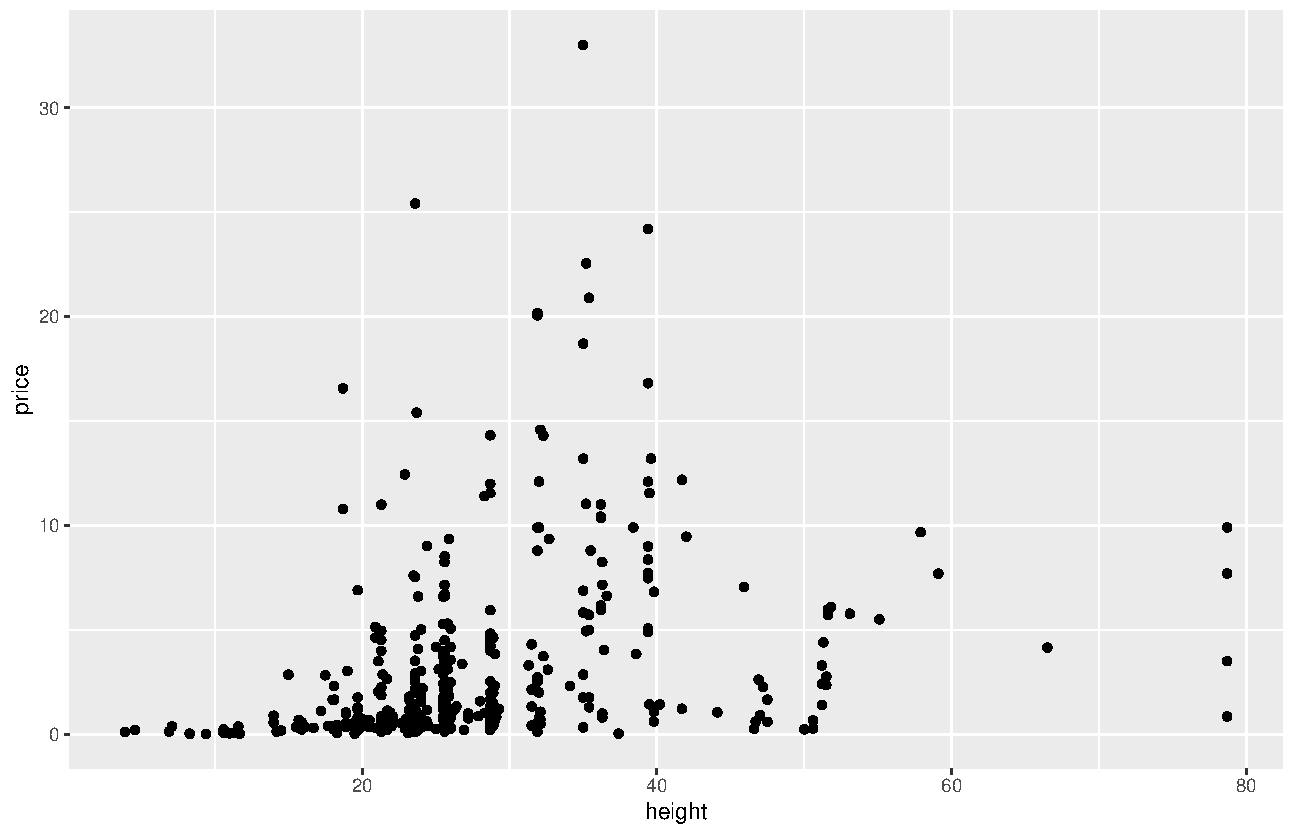
\includegraphics[width=90mm]{pictures/week_10_scatter.pdf}
\end{figure}
}

\frame{
\frametitle{Exercise 1}
Boxplots:
\begin{figure}
\centering
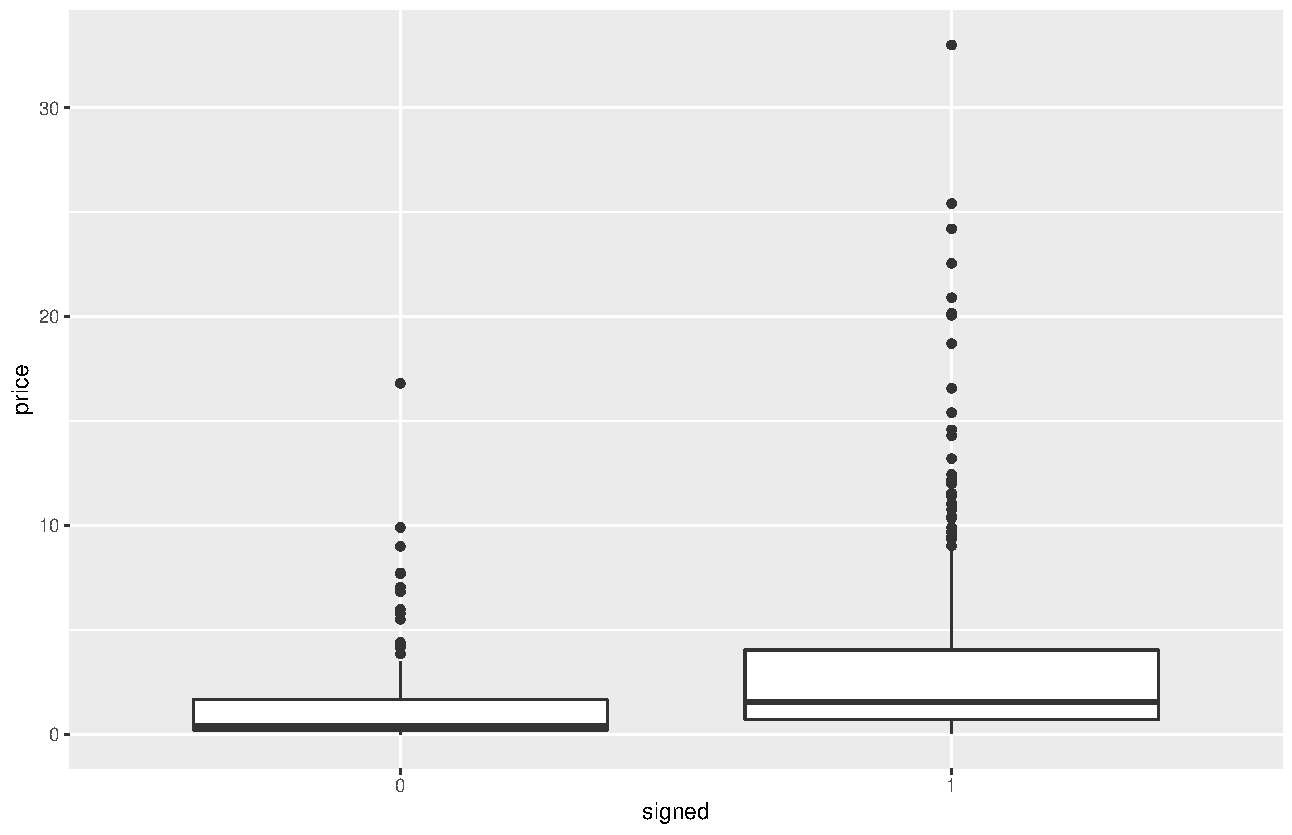
\includegraphics[width=90mm]{pictures/week_10_boxplot.pdf}
\end{figure}
}

\frame{
\frametitle{Exercise 1}
Multivariate:
\begin{figure}
\centering
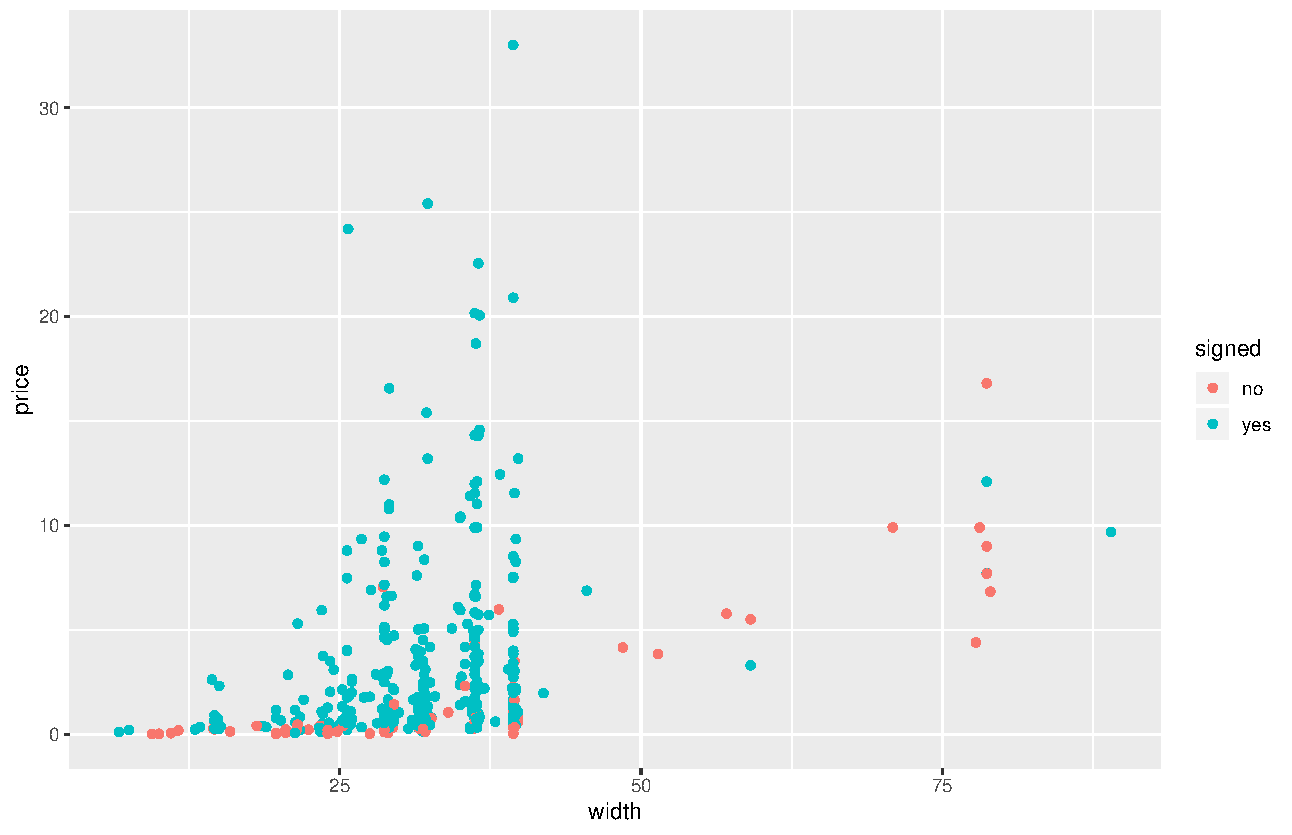
\includegraphics[width=90mm]{pictures/week_10_scatter3.pdf}
\end{figure}
}

\frame{
\frametitle{Exercise 2}
\begin{enumerate}
\item[2.] Propose a theory about what explains the price of a painting \pause
\end{enumerate}
\textbf{Theory} \\
The price of a painting from Monet is explained (determined) by its dimensions: the larger the dimension, the higher the price. \pause

\textbf{Population} \\
The population is represented by the sales of all paintings from Monet. \pause

\textbf{Sample} \\
The sample observations are sales of paintings from Monet from houses number 1, 2, 3.
}

\frame{
\frametitle{Exercise 3}
\begin{enumerate}
\item[3.] Build an appropriate linear model to test your theory \pause
\end{enumerate}
$$Price_i = \beta_0 + \beta_1 Height_i + \beta_2 Width_i + \beta_3 Signed_i + \beta_4 House_i + u_i $$ \pause
Gauss-Markov assumptions make OLS BLUE \citep{Greene}: \pause
\begin{enumerate}
\item Linearity \pause
\item No \textit{perfect} multicollinearity \pause
\item Exogeneity of independent variables, zero-conditional mean (no confounder, no OVB) \pause $ E(u_i | X_1,\ldots,X_k)= 0 $ \pause
\item Observations are i.i.d. \pause
\item Constant variance of the \textit{error} term* (homoskedasticity) \pause
\item Normal distribution of the \textit{error} term* \pause
\end{enumerate}
I could improve my model by including $Width \times Height $ \\ \pause
*\textit{not} necessary
}

\begin{frame}[fragile]
\frametitle{Exercise 4}
\begin{enumerate}
\item[4.] Run your model using your preferred statistical software \pause
\end{enumerate}
In R:
\begin{lstlisting}[language = R]
model <- lm(data = Greene, PRICE ~ HEIGHT + WIDTH + SIGNED + HOUSE)
summary(model)
\end{lstlisting} \pause

In Stata:
\begin{lstlisting}
reg price height width signed house	
\end{lstlisting}
\end{frame}

\frame{
\frametitle{Exercise 4}
OLS can also be computed using matrix algebra: \pause

\begin{itemize}
\item $\textbf{X}$ is the $ n \times k$ matrix of $k-1$ independent variables (the intercept is the $+1$ variable) \pause
\item $\textbf{y}$ is the $n \times 1$ vector with observations of the dependent variable \pause
\item $\textbf{A}'$ is the transpose matrix of $\textbf{A}$ (see math refresher) \pause
\item ${\textbf{A}}^{-1}$ is the inverse of ${\textbf{A}}$: ${\textbf{A}} \times {{\textbf{A}}^{-1}} = \textbf{I}$ (see math refresher) \pause
\end{itemize}

\begin{equation}
\boldsymbol{\hat{\beta}} = {(\textbf{X}' \textbf{X})}^{-1} \textbf{X}' \textbf{y}
\end{equation}
}

\begin{frame}[fragile]
\frametitle{Exercise 4}
Computing OLS using matrix algebra (see R script): \pause

\begin{lstlisting}[language = R]
Y <- Greene$PRICE

X <- matrix(c(rep(1, length(Greene$PRICE)), 
              Greene$HEIGHT, Greene$WIDTH, 
              Greene$SIGNED, Greene$HOUSE),
            ncol = 5, byrow = F)

OLS <- solve(t(X)%*%X) %*% (t(X) %*% Y)
\end{lstlisting} \pause

Outputs: \pause
\begin{lstlisting}[language = R]
            [,1]
[1,] -5.52043300
[2,]  0.09096657
[3,]  0.11169822
[4,]  2.29231727
[5,]  0.38896084
\end{lstlisting}
\end{frame}

\frame{
\frametitle{Exercise 4}
Results from the \texttt{stargazer} package in R \citep{stargazer}:
\begin{table}[!htbp] 
\centering
\resizebox{40mm}{35mm}{
\begin{tabular}{@{\extracolsep{5pt}}lc} 
\\[-1.8ex]\hline 
\hline \\[-1.8ex] 
 & \multicolumn{1}{c}{\textit{Dependent variable:}} \\ 
\cline{2-2} 
\\[-1.8ex] & PRICE \\ 
\hline \\[-1.8ex] 
 HEIGHT & 0.091$^{***}$ \\ 
  & (0.022) \\ 
  & \\ 
 WIDTH & 0.112$^{***}$ \\ 
  & (0.021) \\ 
  & \\ 
 SIGNED & 2.292$^{***}$ \\ 
  & (0.503) \\ 
  & \\ 
 HOUSE & 0.389 \\ 
  & (0.328) \\ 
  & \\ 
 Constant & $-$5.520$^{***}$ \\ 
  & (1.092) \\ 
  & \\ 
\hline \\[-1.8ex] 
Observations & 430 \\ 
Adjusted R$^{2}$ & 0.179 \\ 
F Statistic & 24.395$^{***}$ (df = 4; 425) \\ 
\hline 
\hline \\[-1.8ex] 
\textit{Note:}  & \multicolumn{1}{r}{$^{*}$p$<$0.1; $^{**}$p$<$0.05; $^{***}$p$<$0.01} \\ 
\end{tabular}
}
\end{table} 
}

\frame{
\frametitle{Exercise 4}
Interpretation of the model: \pause
\begin{equation}
	\begin{split}
	Price=-5.520+0.091 Height+0.112 Width \\
	+ 2.292 Signed + 0.389 House + u
	\end{split}	
	\end{equation} \pause
\begin{itemize}
\item \emph{Ceteris paribus}, 1 inch increase in $Height$ ($Width$) raises the price by 0.091 (0.112) units. Similar for the other variables. \pause
\item For each variable the t-test is relative to the null-hypothesis that the true parameter (population parameter) equals 0. \pause
\item We fail to reject the null-hypothesis only for $House$. \pause
\item The theory is not rejected, although our null-hypotheses are $H_0: \beta_i = 0$. \pause One-tailed test would be more appropriate (see script).
\end{itemize}
}

\begin{frame}[fragile]
\frametitle{Exercise 4}
Do you see any problem in your model? \pause

Check the following. In R:
\begin{lstlisting}[language = R]
qplot(x = model$fitted.values, y = model$residuals) + 
  geom_point() + xlab("fitted values") + 
  ylab("residuals") + 
  geom_hline(yintercept = 0, color = c("red"))
\end{lstlisting} \pause

In Stata:
\begin{lstlisting}
rvfplot, yline(0)
\end{lstlisting}
\end{frame}

\frame{
\frametitle{Exercise 4}
What does the following picture suggest to you?
\begin{figure}
\centering
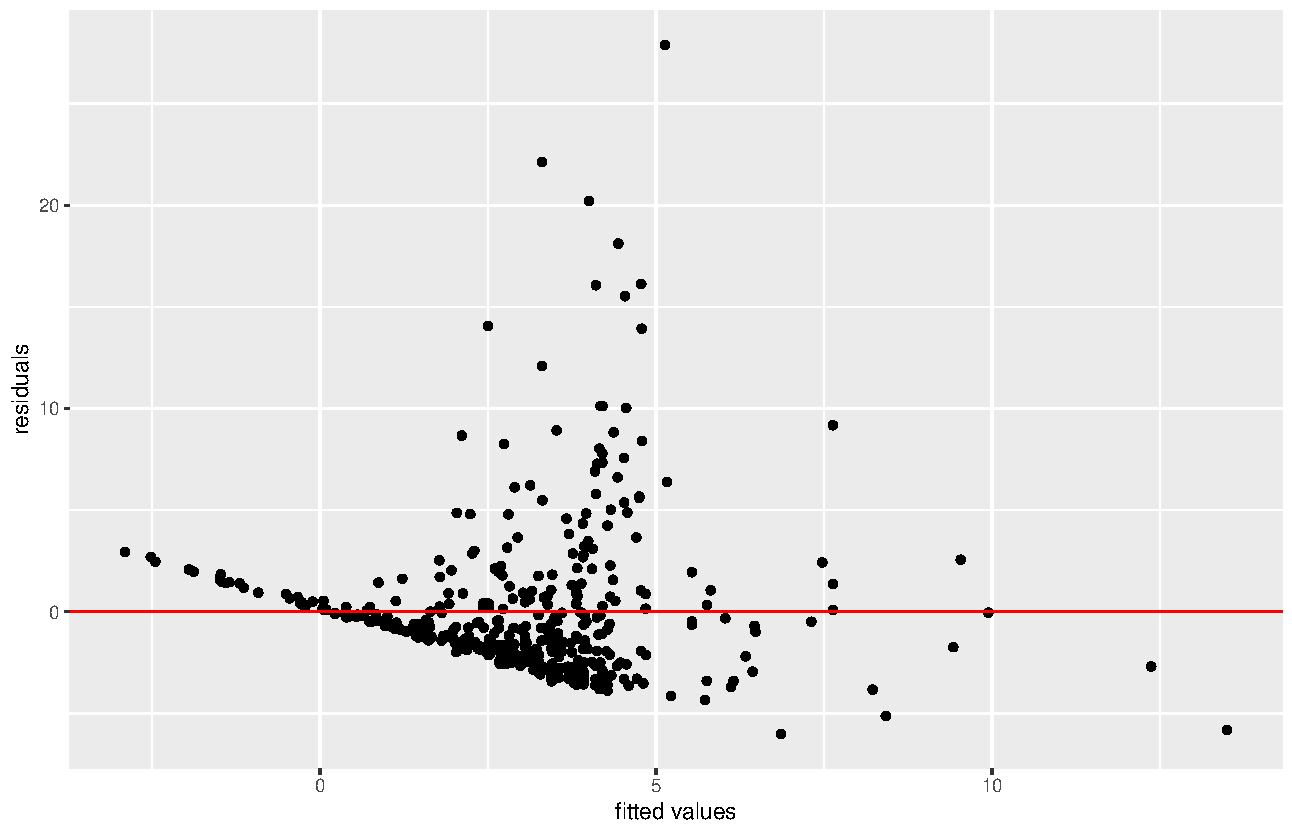
\includegraphics[width=80mm]{pictures/week_10_heteroskedasticity.pdf}
\end{figure} \pause

It is very likely that our \emph{errors} (\textbf{not} residuals) are heteroskedastic. \pause We cannot trust the standard errors of our model.
}

\begin{frame}[fragile]
\frametitle{Exercise 4}
Procedure to have heteroskedasticity-robust estimators for the standard errors (and trustworthy t-tests): \pause

In R:
\begin{lstlisting}[language=R]
library(sandwich)
library(lmtest)
robust <- vcovHC(model, type = "HC1")
coeftest(model, vcov. = robust)
\end{lstlisting} \pause

In Stata:
\begin{lstlisting}
reg price height width signed house, robust
ereturn list r2_a
\end{lstlisting}
\end{frame}

\frame{
\frametitle{Exercise 4}
Heteroskedasticity-robust estimators for the standard errors:
\begin{table}[!htbp] \centering 
\resizebox{40mm}{35mm}{
\begin{tabular}{@{\extracolsep{5pt}}lcc} 
\\[-1.8ex]\hline 
\hline \\[-1.8ex] 
 & \multicolumn{2}{c}{\textit{Dependent variable:}} \\ 
\cline{2-3} 
\\[-1.8ex] & \multicolumn{2}{c}{PRICE} \\ 
 & non-robust & robust \\ 
\\[-1.8ex] & (1) & (2)\\ 
\hline \\[-1.8ex] 
 HEIGHT & 0.091$^{***}$ & 0.091$^{***}$ \\ 
  & (0.022) & (0.022) \\ 
  & & \\ 
 WIDTH & 0.112$^{***}$ & 0.112$^{***}$ \\ 
  & (0.021) & (0.019) \\ 
  & & \\ 
 SIGNED & 2.292$^{***}$ & 2.292$^{***}$ \\ 
  & (0.503) & (0.349) \\ 
  & & \\ 
 HOUSE & 0.389 & 0.389 \\ 
  & (0.328) & (0.289) \\ 
  & & \\ 
 Constant & $-$5.520$^{***}$ & $-$5.520$^{***}$ \\ 
  & (1.092) & (0.939) \\ 
  & & \\ 
\hline \\[-1.8ex] 
Observations & 430 & 430 \\ 
Adjusted R$^{2}$ & 0.179 & 0.179 \\ 
F Statistic (df = 4; 425) & 24.395$^{***}$ & 24.395$^{***}$ \\ 
\hline 
\hline \\[-1.8ex] 
\textit{Note:}  & \multicolumn{2}{r}{$^{*}$p$<$0.1; $^{**}$p$<$0.05; $^{***}$p$<$0.01} \\ 
\end{tabular} 
}
\end{table} 
}

\frame{
\frametitle{Exercise 5}
\begin{enumerate}
\item[5.] How good is your model, jointly considered? \pause
\end{enumerate}
\begin{itemize}
\item An F-test is performed on the model. \pause The F-test compares two nested models: a restricted and an unrestricted one. \pause 
\item We reject the null-hypothesis that the independent variables, \textit{jointly} considered, are not significant in determining the dependent variable. \pause
\item The $R^2$ tells how much of the variance of the observations for the dependent variable is explained by the included regressors. (note: we use the \emph{adjusted} $R^2$)\pause
\item The F-test is a better statistic to evaluate the model, because it is a test which refers to the population. \pause The $R^2$ has no population counterpart: it merely refers to the sample at hand. Thus its meaning is limited.
\end{itemize}
}

\frame{
\frametitle{Exercise 5}

How do we compute the $R^2$? \pause
$$R^2 = {\frac{ESS}{TSS}}={\frac{\sum_{i=1}^{n}{(\hat{y_i}-\bar{y})}^2}{\sum_{i=1}^{n}{(y_i-\bar{y})}^2}={1-\frac{\sum_{i=1}^{n}{\hat{u_i}}^2}{\sum_{i=1}^{n}{(y_i-\bar{y})}^2}}}$$ \pause

How do we perform the $F$ test? \\ \pause
Start from an $F$ distribution with $k-1$ and $n-k$ degrees of freedom ($k$ independent variables, intercept included, $n$ observations). \pause

The critical value ($F$ statistic) from such $F$ distribution is:
$$F[k-1,n-k]=\frac{R^2/(k-1)}{(1-R^2)/(n-k)}$$ 
}

\frame{
\frametitle{Exercise 6}
\begin{enumerate}
\item[6.] Based on your model, predict what would be the price of a painting with arbitrary values for the dependent variables
\end{enumerate}
We can do it with pen and paper, we don't really need a software: \\ \pause
If $Height=30$, $Width=30$, $Signed=0$, $House=3$ then:
\begin{equation}
	\begin{split}
	\hat{Price}=-5.520+0.091 Height+0.112 Width  \\
 + 2.292 Signed + 0.389 House 
	\end{split}	
\end{equation}
\begin{equation}
	\begin{split}
	\hat{Price}=-5.520+0.091 \times 30 +0.112 \times 30  \\
	+ 2.292 \times 0 + 0.389 \times 3 = 1.737
	\end{split}
\end{equation}
}

\frame{
\frametitle{Conclusion}
\begin{center}
All clear? Questions? \\
Thanks and see you next week!
\end{center}
}

\begin{frame}
\bibliographystyle{apalike}
\bibliography{week_10}
\end{frame}

\end{document}